\documentclass{standalone}
\usepackage{tikz}
%------------tikz Setup------------

\tikzstyle{ball} = [circle,shading=ball, ball color=black,
    minimum size=1mm,inner sep=1.3pt]
\tikzstyle{miniball} = [circle,shading=ball, ball color=black,
    minimum size=1mm,inner sep=0.5pt]
\tikzstyle{mminiball} = [circle,shading=ball, ball color=black,
    minimum size=0.6mm,inner sep=0.1pt]
\usetikzlibrary{arrows.meta}
\usetikzlibrary{angles, quotes}
\tikzset{>={Latex[length=2mm,width=1.5mm]}}
\tikzset{->-/.style={decoration={markings, mark=at position #1 with
  {\arrow{>}}},postaction={decorate}}}
\usetikzlibrary{decorations.pathmorphing}
\usetikzlibrary{decorations.pathreplacing}
\usetikzlibrary{arrows.meta,calc}
\usetikzlibrary{bending}
\usetikzlibrary{decorations.markings,shapes.geometric}
\tikzset{->-/.style={decoration={markings, mark=at position #1 with
  {\arrow{>}}},postaction={decorate}}}
\tikzset{-|-/.style={decoration={markings, mark=at position #1 with
  {\arrow{stealth}}},postaction={decorate}}}
\tikzset{movearrow/.style 2 args ={
        decoration={markings,
    mark= at position {#1} with {\arrow{#2}} ,
        },
        postaction={decorate}
    }
}


\begin{document}
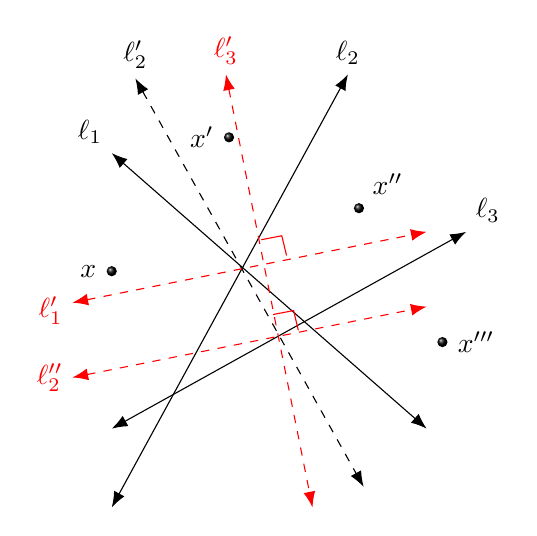
\begin{tikzpicture}
\begin{scope}[scale=1]
    %lines
    \draw [<->] (-2,-1) -- (2.5,1.5);
    \draw [<->] (-2,-2) -- (1,3.5);
    \draw [<->] (-2,2.5) -- (2,-1);
    \draw [<->,dashed] (-1.7,3.45) -- (1.2,-1.74);
    \draw [<->,dashed,red] (-2.5,0.6) -- (2,1.5);
    \draw [<->,dashed,red] (-2.5,-0.35) -- (2,0.55);
    \draw [<->, dashed,red] (-0.55,3.5) -- (0.55,-2);
    %right angles
    \draw[red] (-0.1,1.4) -- (0.16,1.45) -- (0.22,1.2);
    \draw[red] (0.05,0.45) -- (0.31,0.5) -- (0.37,0.25);
    %labels
    \node[above left] at (-2,2.5) {$\ell_1$};
    \node[above] at (1,3.5) {$\ell_2$};
    \node[above right] at (2.5,1.5) {$\ell_3$};
    \node[above] at (-1.7,3.45) {$\ell_2'$};
    \node[left,red] at (-2.5,0.5) {$\ell_1'$};
    \node[left,red] at (-2.5,-0.35) {$\ell_2''$};
    \node[above,red] at (-0.55,3.5) {$\ell_3'$};
    %points
    \node[ball, label={left:$x$}] (x) at (-2,1) {};
    \node[ball, label={left:$x'$}] (x') at (-0.51,2.7) {};
    \node[ball, label={above right:$x''$}] (x'') at (1.14,1.8) {};
    \node[ball, label={right:$x'''$}] (x''') at (2.2,0.1) {};
\end{scope}
\end{tikzpicture}
\end{document}